\chapter{概率论基础}\label{chap:prob}

\begingroup
\newcommand{\B}{\mathscr{B}}
\renewcommand{\F}{\mathscr{F}}
\newcommand{\Exp}{\mathsf{Exp}}
\newcommand{\DExp}{\mathsf{DExp}}
\newcommand{\Lap}{\mathsf{Lap}}

本附录主要介绍Kolmogorov概率论,讨论只局限在数学层面,不涉及概率论的哲学讨论。本附录的连续型随机变量(向量)的讨论需要微积分的基本知识,关于微分学的部分,可以参见\Cref{chap:calculus};积分学我们会在\Cref{sec:expectation} 以数学期望的形式介绍。

\section{从朴素概率论到公理化概率论}

\subsection{Kolmogorov概率论}\label{subsec:kolmogorov-probability}
朴素的概率论通常讨论两种极端的情况,一个是可以用数数的方式来计算概率的情况,比如说掷骰子,另一个是用面积的方式来计算概率的情况,比如在随机选一个圆周上的点。这两个情况分别对应了\textbf{古典概型}和\textbf{几何概型}。

我们先给一些术语。考虑一个随机试验,它的所有可能结果组成的集合称为\textbf{样本空间}\index{样本空间},记为$\Omega$。样本空间的元素称为\textbf{样本点}\index{样本点},通常记为$\omega$. 样本空间的\emph{某些}子集被称为\textbf{事件}。我们来看看这些概念在朴素的概率论中都具体是什么。

\begin{example}[古典概型]
考虑先后掷两个骰子的情况。样本空间为
\[
    \Omega = \{ (i, j): 1 \leq i, j \leq 6 \}.
\]
样本点为$(i, j)$,表示第一个骰子掷出$i$点,第二个骰子掷出$j$点。“第一个骰子掷出$i$点”这个事件可以表示为$A_i = \{ (i, j): 1 \leq j \leq 6 \}$. “第一个骰子掷出$i$点,第二个骰子掷出$j$点”这个事件可以表示为$B_{ij} = \{ (i, j) \}$.
\end{example}

\begin{example}[几何概型]
考虑随机选一个圆周上的点的情况。如果用弧度来表示圆周上的点,那么样本空间为
\[
    \Omega = [0, 2\pi).
\]
样本点为$\omega$,表示选出点的弧度。事件$A = [0, \pi)$表示选出了上半圆周,事件$B = [0, \pi/2)\cup[\pi, 3\pi/2)$表示选出了右上或左下的$1/4$圆周。
\end{example}

那么,如何定义概率呢?朴素地说,概率是某个事件出现的可能性占总可能的比例。

对于古典概型,我们简单认为每个样本点出现的概率都是相同的,也就是说,如果用$p_\omega$表示样本点$\omega$出现的概率,那么对任意$\omega\in\Omega$,都有$p_\omega = 1/|\Omega|$. 于是,对于任意事件$A$,它发生的概率为
\[
    \sum_{\omega\in A} p_\omega = \frac{|A|}{|\Omega|}.
\]
例如在上面掷骰子的例子中,$p_\omega=1/36$,$A$发生的概率为$1/6$,$B$发生的概率为$1/36$.

对于几何概型,不能再用古典概型的方式定义概率。一段长为$2\pi$的圆弧上,一个点的长度当然是$0$,所以选到一个点的概率是$0$。计算选到上半圆周的概率,就是把所有上半圆周上的点的概率加起来,任意多个$0$相加依然还是$0$,所以这样的定义出来的概率永远是零,这样是不可行的。

朴素的直觉告诉我们,选到上半圆周的概率是$1/2$,因为上半圆周刚好占了半个圆周。所以几何概型的概率定义利用了\emph{体积}的概念。事件$A$的概率定义为
\[
    \frac{\text{事件$A$对应的体积}}{\text{样本空间$\Omega$对应的体积}}.
\]
这里体积应该按照广义上来理解,一维集合的体积就是长度,二维集合的体积就是面积,三维集合的体积就是体积,以此类推。例如在上面圆周的例子中,$A$对应的体积(长度)为$\pi$,$\Omega$对应的体积(长度)为$2\pi$,所以$A$发生的概率为$1/2$. 同理,$B$的概率也是$1/2$.

几何概型的定义非常微妙,因为我们并不知道如何定义“体积”。我们来看一个有趣的例子。

\begin{example}[Bertrand悖论]
考虑一个圆,它的半径为$1$. 现在我们随机地在圆上取一个弦,那么这个弦的长度超过$\sqrt{3}$(即圆内接正三角形的边长)的概率是多少?我们给出三种答案。
\begin{enumerate}[label=\textbf{解答\arabic*.},fullwidth,itemindent=2em]
    \item 不妨固定弦的其中一个点$A$,那么另一个点$B$可以在圆上等可能取。以$A$为顶点作圆内接正三角形$ACD$,弦的长度超过$\sqrt{3}$等价于$B$在弧$CD$上,所以概率为$1/3$.
    \item 弦长只与它到圆心的距离有关系,与方向无关。弦长超过$\sqrt{3}$等价于它到圆心的距离小于$1/2$,所以概率为$1/2$.
    \item 弦被它的中点唯一确定,弦长大于$\sqrt{3}$等价于中点落在一个半径为$1/2$的同心小圆内,所以概率为同心小圆面积比上大圆面积,即$(1/2)^2=1/4$.
\end{enumerate}
三种解答的示意图见下(从左到右分别是解答1到3):
\begin{center}
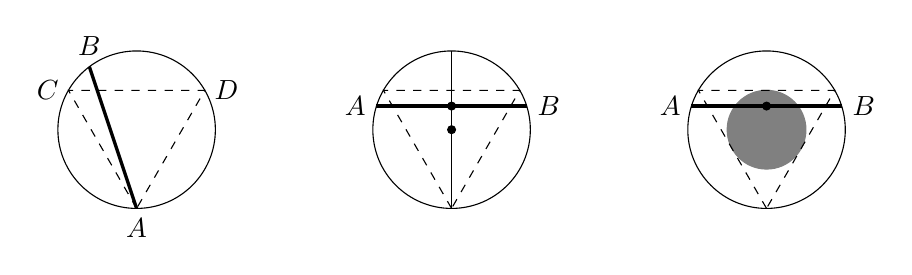
\begin{tikzpicture}
\draw (0,0) circle [radius=1];
\draw[dashed] (0,-1) node[below] {$A$} -- ({-sqrt(3)/2},0.5) node[left] {$C$} -- ({sqrt(3)/2},0.5) node[right] {$D$} -- cycle;
\draw[very thick] (0,-1) -- (-0.6,0.8) node[above] {$B$};

\draw (4,0) circle [radius=1];
\draw (4,-1) -- (4,1);
\draw[dashed] (4,-1)-- ({4-sqrt(3)/2},0.5)  -- ({4+sqrt(3)/2},0.5) -- cycle;
\draw[fill] (4,0) circle [radius=0.05];
\draw[fill] (4,0.3) circle [radius=0.05];
\draw[very thick] ({4-sqrt(1-0.3^2)},0.3) node[left] {$A$} -- ({4+sqrt(1-0.3^2)},0.3) node[right] {$B$};

\draw (8,0) circle [radius=1];
\draw[fill,gray] (8,0) circle [radius=0.5];
\draw[dashed] (8,-1)-- ({8-sqrt(3)/2},0.5)  -- ({8+sqrt(3)/2},0.5) -- cycle;
\draw[fill] (8,0.3) circle [radius=0.05];
\draw[very thick] ({8-sqrt(1-0.3^2)},0.3) node[left] {$A$} -- ({8+sqrt(1-0.3^2)},0.3) node[right] {$B$};
\end{tikzpicture}
\end{center}
\end{example}

因此,我们需要一个更加严格的定义来描述概率。首先注意到,概率应该是一个函数,它的值域是$[0,1]$. 那么,它的定义域应该是什么呢?我们已经看到,概率应该定义在\emph{事件}上,而非\emph{样本点}上。那么,概率可以定义在\emph{任意}事件上吗?这个问题的答案非常微妙,我们不在这里讨论。这里只是指出,我们关心的并不总是任意事件,而是一类被$\sigma$-代数所刻画的事件。

\begin{definition}[$\sigma$-代数]\index{$\sigma$-代数}
设$\Omega$是一个集合,$\F$是$\Omega$的子集的集合。如果$\F$满足
\begin{enumerate}
    \item $\Omega\in\F$;
    \item 如果$A\in\F$,则$A$的补集$\Omega\setminus A\in\F$;
    \item 如果$A_1,A_2,\ldots\in\F$,则$\bigcup_{i=1}^\infty A_i\in\F$.
\end{enumerate}
则称$\F$是$\Omega$上的一个 \textbf{$\sigma$-代数}。
\end{definition}

在样本空间中,我们要求事件也形成一个$\sigma$-代数。这样的$\sigma$-代数称为\textbf{事件域}\index{事件域},记为$\F$,关于这一定义的哲学讨论,可以见\Cref{chap:plausible-reasoning}. 接下来,我们给出Kolmogorov概率论的公理化定义。

\begin{definition}[概率空间,概率测度]\index{概率空间}\index{概率}\index{概率测度}
设$\Omega$是一个集合,$\F$是$\Omega$上的一个$\sigma$-代数。如果函数$\Pr:\F\to[0,1]$满足
\begin{enumerate}
    \item 正则性:$\Pr(\Omega)=1$;
    \item 可列可加性:如果$A_1,A_2,\dots\in\F$是两两不相交的事件,则
    \[
        \Pr\left(\bigcup_{i=1}^\infty A_i\right) = \sum_{i=1}^\infty \Pr(A_i),
    \]
    则称$(\Omega,\F,\Pr)$是一个\textbf{概率空间},$\Pr$称为\textbf{概率测度}或\textbf{概率}。
\end{enumerate}
\end{definition}
容易证明,概率有如下性质:
\begin{proposition}
设$(\Omega,\F,\Pr)$是一个概率空间,则:
\begin{enumerate}
    \item $\Pr(\varnothing)=0$;
    \item 单调性:对任意的$A,B\in\F$,如果$A\subseteq B$,则$\Pr(A)\leq\Pr(B)$;
    \item 有限可加性:对两两不相交的$A_1,A_2,\dots,A_n\in\F$,有
    \[
        \Pr\left(\bigcup_{i=1}^n A_i\right) = \sum_{i=1}^n \Pr(A_i).
    \]
\end{enumerate}
\end{proposition}
他们的证明都不困难,我们略去。

下面我们来看一下之前的古典概型与几何概型都是如何构造概率空间的。

对于古典概型来说,我们容易写出它的概率空间。此时事件域恰好为所有$\Omega$的子集的集合,概率测度的定义也就是我们之前的定义:$\Pr(A)=|A|/|\Omega|$. 

对于几何概型来说,概率空间最大的困难在于事件域和概率测度的定义。为了简化讨论,我们集中在$\Omega=[0,1]^n$,也就是$n$维立方体的情况。我们知道,对于一个长方体
\[\prod_i(a_i,b_i)=\{x=(x_1,x_2,\ldots,x_n)\in\R^n:a_i<x_i<b_i\},\]
它的体积为$\prod_i(b_i-a_i)$. $\Omega$上事件域至少应该包含所有长方体,所以我们就定义事件域为包含所有长方体的最小$\sigma$-代数$\B([0,1]^n)$。换言之,如果还有一个$\sigma$-代数$\F$包含所有长方体,那么$\B([0,1]^n)\subseteq\F$. 我们将这一$\sigma$-代数称为\textbf{Borel代数}\index{Borel代数}. Borel代数包含了绝大部分我们要讨论的集合,例如开集、闭集、单点集、有限集、可数集等,可以简单归纳为“合理的集合”。

事件域的定义已经给出,我们还需要定义概率测度。概率测度$\Pr$的第一个要求是,让正方体的概率等于它的体积。第二个要求是平移不变性,也就是说,如果$A\in\B([0,1]^n)$,那么对任意的$x\in\R^n$,定义$A+x=\{y\in\R^n:y=x+z,z\in A\}$,只要$A\in\B([0,1]^n)$,就有$\Pr(A+x)=\Pr(A)$. 这样的概率测度是存在且唯一的,我们称之为\textbf{Lebesgue测度}\index{Lebesgue测度},常记为$\lambda$.

注意,Borel代数和Lebesgue测度的定义可以不局限在$[0,1]^n$,他们可以定义在与实数相关的各种空间上。在本附录中,我们最主要是用的是$\R^n$上的相关定义,例如$\B(\R^n)$就是包含所有$n$维开长方体(每条边是开区间)的最小$\sigma$-代数,$\lambda$就是定义在$\B(\R^n)$上的Lebesgue测度. $\R^n$上的Lebesgue测度其实是概率测度的扩展(而非概率测度),因为此时不再要求有正则性(即$\lambda(\Omega)=1$),但额外要求$\lambda(\varnothing)=0$.

\subsection{条件概率,独立性}
接下来,我们讨论条件概率与独立性。我们还是看先后掷两个骰子的例子。如果掷完第一个骰子,我们马上观察结果,然后再掷第二个骰子,问第一个骰子是$i$,第二个是$j$的概率是多少?如果继续套用原来的概率空间,我们很快就会觉得不对劲。此时,第一个骰子完全没有随机性!所以朴素的直觉告诉我们,这里的概率应该有另一个依赖于第一次投骰子结果的定义,这样的概率就是\emph{条件概率}。

我们直接给出一般情况下条件概率的定义。

\begin{definition}[条件概率]\index{条件概率}
设$(\Omega,\F,\Pr)$是一个概率空间,$A,B\in\F$是两个事件,且$\Pr(A)>0$. 则称
\[
    \Pr(B|A) = \frac{\Pr(A\cap B)}{\Pr(A)}
\]
是事件$B$在事件$A$发生的条件下发生的\textbf{条件概率}。
\end{definition}

以上定义要求$A$发生概率为正,然而$A$是零概率的时候也是可能有条件概率的。例如,
从$[0,1]\times[0,1]$中均匀地随机选一个点$(X,Y)$,观察它的横坐标$X$,不管什么样的$x$,$X=x$的概率都是$0$。然而,从朴素的直觉来看,条件在$X=x$上,$Y>1/2$的概率不仅存在,而且应该是$1/2$。在\Cref{sec:random-variable} 中,我们会针对一类特殊的事件,给出此时条件概率的定义。

我们继续看投两个骰子的例子。假设事件$A$是“第一个骰子是$i$“,事件$B$是“第二个骰子是$j$”。我们可以计算出$\Pr(B|A)=\Pr(B)=\frac{1}{6}$. 如果单看数学计算,这是一个非常神奇的式子:条件在$A$上和不条件在$A$上概率是一样的!从朴素的直觉来说,这件事情却并不神秘,因为第一个骰子的结果和第二个骰子的结果是不应该有关系的。我们把这种现象称为\textbf{独立性}。更一般地,对任意事件$A,B$,如果$\Pr(A)>0$,那么
\[\Pr(B|A)=\Pr(B)\iff \frac{\Pr(A\cap B)}{\Pr(A)}=\Pr(B)\iff \Pr(A\cap B)=\Pr(A)\Pr(B).\]
最后一个式子并不要求$\Pr(A)>0$,因此我们用它作为独立性的定义,这样定义可以不依赖条件概率。

\begin{definition}[独立性]\index{独立性}
设$(\Omega,\F,\Pr)$是一个概率空间,$A,B\in\F$是两个事件。如果$\Pr(A\cap B)=\Pr(A)\Pr(B)$,则称事件$A$和$B$\textbf{相互独立}。

一般地,给定一个事件族$\mathscr{A}\subseteq\F$,如果对任意的有限个不同的$A_1,A_2,\ldots,A_n\in\mathscr{A}$,都有
\[
    \Pr\left(\bigcap_{i=1}^n A_i\right) = \prod_{i=1}^n \Pr(A_i),
\]
则称事件族$\mathscr{A}$中的事件是\textbf{相互独立}的。
\end{definition}

我们在定义中还给出了多个事件相互独立的定义,这一定义是说不管挑出其中多少个事件,他们都应该满足交的概率等于概率的积。这并不等价于任意两个事件都相互独立,我们看下面的例子。

\begin{example}
两个人进行石头剪刀布游戏,每个人独立等概率地出剪刀石头布. 考虑下面三个事件:$A=\{\text{甲出了石头}\}$,$B=\{\text{乙出了剪刀}\}$,$C=\{\text{甲赢}\}$.

容易算出,$\Pr(A\cap B)=\Pr(A)\Pr(B)=1/9$,$\Pr(A\cap C)=\Pr(A)\Pr(C)=1/9$,$\Pr(B\cap C)=\Pr(B)\Pr(C)=1/9$,所以$A,B,C$两两独立. 但是$A,B,C$不是相互独立的:$\Pr(A\cap B\cap C)=1/9\neq 1/27=\Pr(A)\Pr(B)\Pr(C)$.
\end{example}

这个例子说明,三个事件的独立性远比他们任意两个之间的独立性要复杂,三个事件可能放在一起才会出现不独立的情况。对于一般情况,这样的现象更加普遍,所以我们多个事件的独立性定义是要求任意有限个事件都独立,而不是任意两个事件都独立。

最后,我们给出条件概率的一些性质。

\begin{proposition}\label{prop:conditional-probability}
设$(\Omega,\F,\Pr)$是一个概率空间,那么
\begin{enumerate}
    \item 对任意$A\in\F$满足$\Pr(A)>0$,$\Pr(\cdot|A)$也是一个概率测度;
    \item $\Pr(|\Omega)=\Pr(\cdot)$,
    \item 对任意$A\in\F$满足$\Pr(A)>0$,$\Pr(A|A)=1$.
\end{enumerate}
\end{proposition}
以上性质的证明都很简单,我们就不给出了。

\begin{theorem}[全概率公式]\index{全概率公式}\label{thm:total-probability}
设$(\Omega,\F,\Pr)$是一个概率空间,$A_1,A_2,\ldots\in\F$是一列两两不相交的事件,且$\Pr(A_i)>0$,$\bigcup_{i=1}^\infty A_i=B$,则对任意的$C\in\F$,有
\[
    \Pr(C|B) = \sum_{i=1}^\infty \Pr(C|A_i)\Pr(A_i).
\]
特别地,对于有限个$A_i$,这一定理也成立。
\end{theorem}
\begin{proof}
注意到
\[
    \Pr(C) = \Pr(C\cap B) = \Pr\left(C\cap\bigcup_{i=1}^\infty A_i\right) = \Pr\left(\bigcup_{i=1}^\infty (C\cap A_i)\right) = \sum_{i=1}^\infty \Pr(C\cap A_i).
\]
最后一个等号是因为$C\cap A_i$两两不相交。另一方面,
\[
    \Pr(C\cap A_i) = \Pr(C|A_i)\Pr(A_i),
\]
所以
\[
    \Pr(C) = \sum_{i=1}^\infty \Pr(C|A_i)\Pr(A_i).
\]
对于有限个$A_i$,只需要把无穷求和改成有限求和,利用有限可加性即可即可。
\end{proof}

全概率公式是一种分而治之的思想,它把一个复杂的事件分解成若干个简单的事件,然后再把简单的事件的概率加起来。我们来看一个例子。

\begin{example}
    从装有$w$个白球和$b$个黑球的盒子中随机地取出一个球,不放回,再取出一个球。问第二个球是白球的概率是多少?

    设事件$A$是“第一个球是白球”,事件$B$是“第二个球是白球”。我们有
\begin{align*}
    \Pr(B) &= \Pr(B|A)\Pr(A) + \Pr(B|\bar{A})\Pr(\bar{A}) \\
    &=\frac{w-1}{w+b-1}\cdot\frac{w}{w+b} + \frac{w}{w+b-1}\cdot\frac{b}{w+b}\\
    &=\frac{w}{w+b}.
\end{align*}
    这里$\bar A$指的是$A$的补集,即“第一个球是黑球”。
\end{example}

\begin{theorem}[贝叶斯公式]\index{贝叶斯公式}\label{thm:bayes}
设$(\Omega,\F,\Pr)$是一个概率空间,$A,B\in\F$且$\Pr(A),\Pr(B)>0$,则
\[
    \Pr(A|B) = \frac{\Pr(B|A)\Pr(A)}{\Pr(B)}.
\]
\end{theorem}
这一公式的证明几乎是显然的,我们略去。

一个特别重要的推论被称为\emph{链式法则}\index{链式法则},它是\emph{Bayes网络}\index{Bayes网络}的基础。

\begin{corollary}[链式法则]\index{链式法则}\label{cor:chain-rule}
设$(\Omega,\F,\Pr)$是一个概率空间,$A_1,A_2,\ldots,A_n\in\F$,且$\Pr(A_1\cap A_2\cap\cdots\cap A_n)>0$,则
\begin{align*}
    &\Pr(A_1\cap A_2\cap\cdots\cap A_n)\\
    = &\Pr(A_1)\Pr(A_2|A_1)\Pr(A_3|A_1\cap A_2)\cdots\Pr(A_n|A_1\cap A_2\cap\cdots\cap A_{n-1}).
\end{align*}
\end{corollary}

我们也看一个例子。

\begin{example}[P\'olya的罐子]
    一个罐子装有$w$个白球和$b$个黑球,随机取出一个,观察它的颜色,放回,再放回相同颜色的$c$个球,再随机取一次,重复上述操作,如此反复$n$次,问每一次都取到白球的概率是多少?

    设事件$A_i$是“第$i$次取出的球是白球”。我们有
\begin{align*}
    \Pr(A_1)&=\frac{w}{w+b},\\
    \Pr(A_2|A_1)&=\frac{w+c}{w+b+c},\\
    \Pr(A_3|A_1\cap A_2)&=\frac{w+2c}{w+b+2c},\\
    &\cdots\\
    \Pr(A_n|A_1\cap A_2\cap\cdots\cap A_{n-1})&=\frac{w+nc}{w+b+nc}.
\end{align*}
    所以
\[
    \Pr(A_1\cap A_2\cap\cdots\cap A_n) = \frac{w}{w+b}\cdot\frac{w+c}{w+b+c}\cdots\frac{w+nc}{w+b+nc}.
\]
\end{example}

\begin{remark}
    在概率论中,我们经常要讨论事件的交,所以我们通常会把$A\cap B$简记为$AB$。此外,事件不相交我们也称之为\textbf{互斥}。事件$A$的补事件,即$\Omega\setminus A$.我们会记为$\bar{A}$或$A^c$.
    
    另外,我们也经常要讨论一个关于$\omega$的陈述$Q(\omega)$定义的事件$\{\omega\in\Omega:Q(\omega)\}$,在P\'olya的罐子的例子中,事件$A_1$其实就是由陈述$Q(\omega)$:“$\omega$中第一次取出的球是白球”定义的事件。在这种情况下,我们将这一事件简记为$\{Q\}$,它的概率就是$\Pr(\{Q\})$或者简记为$\Pr(Q)$。此时,事件交的概率也经常以逗号的形式写出,例如,$\Pr(A_1A_2)$我们会记为$\Pr(\text{第一次取出的球是白球},\text{第二次取出的球是白球})$. 这样的记号更直观,并且在随机变量部分会经常使用。
\end{remark}
\section{随机变量,分布函数}\label{sec:random-variable}

接下来,我们讨论随机变量。从某种意义上说,随机变量是另一种刻画概率测度的手段。然而,随机变量能够更加直观、定量描述概率空间中的事件,所以这是一个更加容易使用的概念。

\subsection{基本定义}

为了理解随机变量的概念,我们依然从古典概型入手。

\begin{example}\label{ex:random-variable}
继续考虑先后投两个骰子的情况,假设它的概率空间是$(\Omega,\F,\Pr)$,他们的定义我们在\Cref{subsec:kolmogorov-probability} 的末尾已经讨论过了。

我们可以定义一个从样本空间$\Omega$到$\N$的函数$S(i,j)=i+j$,也就是两个点数的和。我们来看看$S$与事件域的关系。$\{S=s\}=\{(i,j)\in\Omega:i+j=s\}$,所以$S$将原本的事件精简成了一个数字。这个过程丢弃了一些事件,例如$S$无法表达事件$\{(1,2)\}$,实际上,它无法区分$(1,2)$和$(2,1)$,它把这两个样本点都看成了$3$. 但是,$S$仍然保留了很多信息,例如,$S$可以区分事件$\{(1,1)\}$和$\{(2,2)\}$,它们分别对应$2$和$4$. 总结来说,$S$将原本更精细的事件域压缩成了更粗糙的事件域。

有了上面的感觉,我们可以看一个更抽象的函数。定义一个从样本空间$\Omega$到$\N^2$的函数$X$,它的定义为$X(i,j) = (i,j)$. 换句话说,它把样本点看成一个$\N^2$的元素。$\F$中的所有事件都可以表达为$\{X\in B\}$,这里$B\subseteq\N^2$. 所以$X$完全刻画了整个事件域。
\end{example}

上面例子中的$S$和$X$都是\emph{随机变量}的例子。我们给出随机变量的定义。

\begin{definition}[随机变量,随机元]\index{随机变量}\index{随机元}
设$(\Omega,\F,\Pr)$是一个概率空间,$X:\Omega\to\R$是一个函数。如果对任意的$x\in\R$,$\{X\in\B(\R)\}\in\F$,则称$X$是一个\textbf{随机变量}. 

一般地,考虑一个集合$S$以及其上的$\sigma$-代数$\F_S$,$X:\Omega\to S$是一个映射。如果对任意的$A\in\F_S$,$\{X\in A\}\in\F$,则称$X$是一个\textbf{随机元}。如果$S=\R^n$且$\F_S=\B(\R^n)$,则称$X$是一个\textbf{$n$维随机向量}。
\end{definition}

下面对这个定义做一些说明。首先,随机变量是一个映射,而不是一个数字,这一点经常会被人误解。直观上说,它是一个映射是因为,它的值是随机的,背后有一个未知的力量在抛硬币,我们把从抛硬币到观测值这一整个东西称之为随机变量。

定义的后面还涉及了$\sigma$-代数相关的东西,我们也给一个简要说明。Borel代数包含了“合理的集合”,所以$\{X\in\B(\R)\}$表示事件“$X$取合理的值”。随机变量的要求其实就是,“$X$取合理的值”是一个我们可以定义概率的事件。

我们下面讨论一些随机变量的基本性质。

\begin{proposition}\label{prop:random-variable}
设$(\Omega,\F,\Pr)$是一个概率空间,$X:\Omega\to\R$是一个随机变量. 假设函数$g:\R\to\R$是一个连续函数,则$g(X)=g\circ X$也是一个随机变量。更一般地,如果$X:\Omega\to\R^n$是一个随机向量,$g:\R^n\to\R^m$是一个连续函数,则$g(X)=g\circ X$也是一个随机向量。
\end{proposition}

这一性质告诉我们了一种构造随机变量的方式,我们可以先构造一个随机变量,然后对它进行一些连续的操作,例如加减乘除、取指数、取对数、取幂等等,这样得到的新的函数也是一个随机变量。

实际上,不连续的函数进行复合也可以构造新的随机变量,这样的函数可以用\textbf{Borel函数}\index{Borel函数}来刻画。实际上,Borel函数就是样本空间$\R^n$上的随机向量。


接下来,我们进入分布函数的讨论。我们说过,随机变量某种意义上给出了概率测度的另一种刻画方式,而这一桥梁就是由分布函数给出的。

考虑概率空间$(\Omega,\F,\Pr)$,以及一个随机变量$X:\Omega\to\R$. 要刻画概率测度$\Pr$,我们需要给出所有的事件$A\in\F$的$\Pr(A)$。如果$A$可以被写成$\{X\in B\}$的形式,那么我们可以用$\Pr(X\in B)$来刻画$\Pr(A)$. 而我们之前说过,要确定$\Pr(X\in B)$,基本上只需要确定$\Pr(X\in(a,b))$。这一概率还是有两个未定元$a,b$,所以更简便的方式是确定$F_X(b)=\Pr(X\in(-\infty,b])$,容易证明,开区间的概率完全可以由$F_X(b)$给出,所以$F_X$完全刻画了$\Pr$. 更一般地,我们有如下定义。

\begin{definition}[分布函数]\index{分布函数}
设$(\Omega,\F,\Pr)$是一个概率空间,$X:\Omega\to\R$是一个随机变量。定义函数$F_X:\R\to\R$为$F_X(x) = \Pr(X\leq x)$. 我们称$F_X$是$X$的\textbf{分布函数},记作$X\sim F$.

如果$X:\Omega\to\R^n$是一个随机向量,定义函数$F_X:\R^n\to\R$为$F_X(x) = \Pr(X\leq x)$,这里$X\leq x$是指对任意的$i=1,2,\ldots,n$,都有$X_i\leq x_i$. 我们称$F_X$是$X$的\textbf{分布函数},记作$X\sim F$.
\end{definition}

容易验证,分布函数具有如下的性质:

\begin{proposition}\label{prop:distribution-function}
设$(\Omega,\F,\Pr)$是一个概率空间,$X:\Omega\to\R$是一个随机变量,$F_X$是它的分布函数,则
\begin{enumerate}
    \item $F_X$是一个非减函数;
    \item $\lim_{x\to-\infty}F_X(x)=0$,$\lim_{x\to+\infty}F_X(x)=1$;
    \item $F_X$是右连续的,即对任意的$x\in\R$,都有$\lim_{y\downarrow x}F_X(y)=F_X(x)$;
    \item $F_X$在每一点处的左极限存在,即对任意的$x\in\R$,都有$F(x-)=\lim_{y\uparrow x}F_X(y)$存在.
\end{enumerate}
\end{proposition}

实际上,分布函数也可以由上面四条给出定义,这是因为,满足上面四条性质的函数恰好是某个随机变量的分布函数:

\begin{theorem}\label{thm:distribution-function}
设$F$是$\R^n\to\R$的函数,满足\Cref{prop:distribution-function} 的四条性质. 

在概率空间$([0,1]^n,\B([0,1]^n),\lambda)$上,存在一个随机变量$X$,使得$F_X=F$.
\end{theorem}

所以,我们今后也称呼满足\Cref{prop:distribution-function} 四条性质的函数为分布函数。

我们看一个分布函数计算概率的简单例子。

\begin{example}\label{ex:distribution-prob}
考虑$\R$上的分布函数$F$,它由随机变量$X$定义。那么,
\begin{itemize}
    \item $\Pr(X\leq a)=F(a)$,
    \item $\Pr(X<a)=F(a-)$,
    \item $\Pr(X>a)=1-F(a)$,
    \item $\Pr(X\geq a)=1-F(a-)$,
    \item $\Pr(X=a)=F(a)-F(a-)$。
\end{itemize}
\end{example}

如果我们就限制在空间$([0,1]^n,\B([0,1]^n),\lambda)$上,随机变量几乎就等同于分布函数。现在,我们将分布函数与概率测度联系在一起:

\begin{theorem}\label{thm:uniqueness-of-distribution-function}
设$F:\R^n\to\R$是一个分布函数,则在$\R^n$以及$\B(\R^n)$上,存在唯一的概率测度$\Pr$,使得对任意$a_i\leq b_i$,
\[
    \Pr\left(\prod_{i=1}^n(a_i,b_i]\right) = \prod_{i=1}^n (F(b_i)-F(a_i)).
\]
\end{theorem}

特别地,分布函数
\[F(x)=\begin{cases}
    0,&x<0,\\
    x,&0\leq x\leq 1,\\
    1,&x>1.
\end{cases}\]
对应的概率测度就是我们之前讨论的$[0,1]$上的Lebesgue测度\index{Lebesgue测度}.

根据上面的讨论,分布函数的特性决定了随机变量的特性。根据分布函数的不同性质,我们可以将随机变量分为不同的类型。下面我们将讨论一些重要的类别。

\subsection{离散型随机变量}\index{随机变量!离散型~}

我们首先讨论\emph{离散型随机变量}。离散型随机变量的分布函数$F$称之为\emph{离散型分布}\index{分布!离散型~},它是一个阶梯函数,它的函数值只在有限或者可数个点$x_1,x_2,\dots$上发生跳变,在$x_i$的跳变为$p_i=F(x_i)-F(x_i-)$。这一分布函数对应的概率测度$\Pr$我们称之为\emph{离散型测度}\index{测度!离散型~},这种测度集中在$x_i$上,即$\Pr(X=x_i)=p_i$。分布函数形如下图:

\begin{center}
\begin{tikzpicture}
\draw[->] (-2,0) -- (5,0) node[right] {$x$};
\draw[->] (0,0) -- (0,3) node[above] {$F(x)$};
\draw[->,very thick] (-2+0.2,0) -- (-1,0) circle [radius=0.05];
\draw[dashed] (-1,0) -- node[left] {$p_1$} (-1,1);
\draw[->,very thick] (-1,1) --  (1,1) circle [radius=0.05];
\draw[dashed] (1,1) -- node[left] {$p_2$} (1,2);
\draw[->,very thick] (1,2) -- (3,2) circle [radius=0.05];
\draw[dashed] (3,2) -- node[left] {$p_3$} (3,2.5);
\draw[->,very thick] (3,2.5) -- (5-0.2,2.5);
\draw (-1,0) node[below] {$x_1$};
\draw (1,0) node[below] {$x_2$};
\draw (3,0) node[below] {$x_3$};
\end{tikzpicture}
\end{center}

离散型分布可以由分布列给出,分布列是一个序列$p_1,p_2,\dots$,其中$p_i=\Pr(X=x_i)$,且$\sum_{i=1}^\infty p_i=1$.

\Cref{tab:discrete-distribution} 列举了一些本书中用到的离散型分布,他们都是整数取值,所以我们记$p_i=\Pr(X=i)$.

\begin{table}[htbp]
\centering
\begin{tabular}{cccc}
\toprule
名称 & 符号 & 分布列 & 参数 \\
\midrule
离散均匀\index{分布!离散均匀~} & $\U[n]$ &$p_i=1/n$,$i=1,\dots,n$ & $n\in\N$ \\
Bernoulli\index{分布!Bernoulli~} & $B(1,p)$ & $p_1=p$,$p_0=1-p$ & $p\in[0,1]$ \\
对称Bernoulli\index{分布!对称Bernoulli~} & — &$p_1=p_{-1}=1/2$ & — \\
二项\index{分布!二项~} &$B(n,p)$ &$p_k=\binom{n}{k}p^k(1-p)^{n-k}$ & $n\in\N$,$p\in[0,1]$ \\
\bottomrule
\end{tabular}
\caption{本书中用到的离散型分布}
\label{tab:discrete-distribution}
\end{table}

\subsection{连续型随机变量}\index{随机变量!连续型~}

我们再来讨论\emph{连续型随机变量},连续型随机变量的分布函数$F$称为\emph{连续型分布}\index{分布!连续型~},对应的概率测度$\Pr$称之为\emph{绝对连续测度}\index{测度!绝对连续~}. 从名字上就可以看出,测度才是定义连续型随机变量的关键。我们给出绝对连续测度的定义。

\begin{definition}[绝对连续测度]\index{测度!绝对连续~}
$\R$上的测度$\Pr$称为\textbf{绝对连续测度},如果对任意$\epsilon>0$,存在$\delta>0$使得任意$A\in\B(\R)$满足$\lambda(A)<\delta$,都有$\Pr(A)<\epsilon$.
\end{definition}

直观上说,绝对连续测度的意思是当体积$\lambda(\cdot)$发生微小变化的时候(变化量为$\lambda(A)$),测度$\Pr(\cdot)$也只发生微小的变化(变化量为$\Pr(A)$),这和通常函数连续的定义并没有太大的区别。

那么,绝对连续测度对应的是连续分布函数吗?答案是否定的,绝对连续测度对应的分布函数有相当漂亮的一种刻画方式:

\begin{theorem}[Lebesgue微分定理]\label{thm:lebesgue-differentiation-theorem}
设$F:\R\to\R$是绝对连续测度对应的分布函数,那么
\[\lambda(\{x\in\R:F'(x)\text{ 不存在}\})=0.\]
定义函数:
\[f(x)=\begin{cases}
    F'(x),&F'(x)\text{ 存在},\\
    0,&\text{其他}.
\end{cases}\]
则$f$是一个非负可积函数,且对任意的$a<b$,都有
\begin{equation}
    F(b)-F(a) = \int_a^b f(x)\d x.\label{eq:Newton-Leibniz}
\end{equation}
\end{theorem}
此处的积分可以理解为Riemann积分或者后面\Cref{sec:expectation} 中的Lebesgue积分。

\Cref{thm:lebesgue-differentiation-theorem} 意味着,绝对连续测度对应的分布函数几乎处处可以求导,并且所得到的导函数积分回去还是原来的分布函数。这样的函数我们称之为\emph{绝对连续函数}\index{绝对连续函数}.

那么,这个$f$应该如何理解呢?先不管\Cref{thm:lebesgue-differentiation-theorem},回到绝对连续测度,仿照导数的定义,考虑极限
\[\frac{\d\Pr}{\d\lambda}(x)=\lim_{\lambda(A)\to 0,x\in A}\frac{\Pr(A)}{\lambda(A)},\]
也就是点$x$附近$\Pr(\cdot)$的微小变化相对于$\lambda(\cdot)$的微小变化.

那么,给定一个集合$A$,要如何求$\Pr(A)$?按照微积分的朴素直观,我们应该将$\Pr$微小的变化转变为$\lambda$微小的变化,也就是积分:
\[\Pr(A)=\int_{x\in A}\frac{\d\Pr}{\d\lambda}(x)\d\lambda(x).\]
我们可以把\eqref{eq:Newton-Leibniz} 改写成如上的形式:
\[\Pr((a,b])=\int_{x\in (a,b]}f(x)\d x.\]
在一维的情况下,$x$的微小变化就是$\lambda(x)$的微小变化,所以$\d x=\d\lambda(x)$。综合这两点,我们容易相信,
\[f(x)=\frac{\d\Pr}{\d\lambda}(x)\iff \d\Pr=f(x)\d\lambda.\]
所以,$f$应该理解为“密度”。打个比方,$\lambda$是物体的体积,$\Pr$是物体的质量,那么$f$就是这个物体每个很小的部分上的体积质量除以体积,也就是密度。所以,我们将$f$称之为\textbf{概率密度函数}\index{概率密度函数},或者简称\textbf{密度}。通常,$X$的密度记作$p_X$。

那么,概率测度和密度的区别是什么呢?对于刚接触概率论的人来说,似乎很难理解他们之间的区别。比如说,他们会写$p(X=x)$甚至$\Pr(X=x)$来表示密度在$x$处的值$p(x)$,又或者,用$\int\Pr(X=x)\d x$来表示对密度的积分。这些当然都是不对的,我们下面慢慢论述。

首先,根据\Cref{thm:lebesgue-differentiation-theorem},$F$是连续函数,所以根据\Cref{ex:distribution-prob},$\Pr(X=x)=F(x)-F(x-)=F(x)-F(x)=0$. 所以$\Pr(X=x)$根本就是零,它和密度函数没有任何关系,所以上面这些写法都是错的。

那么,要怎么理解密度$p(\cdot)$和概率测度$\Pr(\cdot)$的区别呢?当然,从定义的角度他们就完全不同:一个是从实数到实数的映射,一个是从实数的集合到实数的映射。但是这样的区别对于初学者来说并不直观。最直观的区别就在于密度这一词:虽然铅很重(密度大),但是几亿倍于铅体积的棉花却应该比铅重。所以,密度是微观的,刻画很小部分集合的概率值,也就是$\d\Pr=p\d \lambda$;而概率刻画的是宏观的,计算任何一个集合的概率,也就是$\Pr(A)$.

\begin{remark}
    上面的记号$\d\Pr/\d\lambda$并不是随意写出来的,我们叫它导数也不是随意的。在测度论中,\Cref{thm:lebesgue-differentiation-theorem} 可以被推广为\textbf{Radon-Nikodym定理}\index{Radon-Nikodym定理},这一定理直接保证了形如$\d\Pr/\d\lambda$的函数的存在性,这一函数被称之为\textbf{Radon-Nikodym导数}\index{Radon-Nikodym导数}。
\end{remark}

利用密度,我们可以很容易计算概率:
\begin{proposition}\label{prop:continuous-prob}
设$X$是一个连续型随机变量,$f$是它的密度函数,则对任意的$B\in\B(\R)$,都有
\[\Pr(X\in B)=\int_{x\in B}f(x)\d x.\]
\end{proposition}

在\Cref{tab:continuous-distribution} 中,我们给出本书中用到的一些连续型分布的密度函数。

\begin{table}[htbp]
\centering
\begin{tabular}{cccc}
\toprule
名称 & 符号 & 密度函数 & 参数 \\
\midrule
连续均匀\index{分布!连续均匀~} & $\U(a,b)$ &$p(x)=\frac{1}{b-a}$,$x\in[a,b]$ & $a<b$ \\
指数\index{分布!指数~} & $\Exp(\lambda)$ & $p(x)=\lambda e^{-\lambda x}$,$x\geq 0$ & $\lambda>0$ \\
双指数\index{分布!双指数~} & $\DExp(\lambda)$ & $p(x)=\frac{\lambda}{2}e^{-\lambda|x|}$,$x\in\R$ & $\lambda>0$ \\
Laplace\index{分布!Laplace~} & $\Lap(\mu,\lambda)$ & $p(x)=\frac{\lambda}{2}e^{-\lambda|x-\mu|}$,$x\in\R$ & $\mu\in\R$,$\lambda>0$ \\
正态(Gauss)\index{分布!正态~}\index{分布!Gauss~} & $\Nor(\mu,\sigma^2)$ & $p(x)=\frac{1}{\sqrt{2\pi}\sigma}e^{-\frac{(x-\mu)^2}{2\sigma^2}}$,$x\in\R$ & $\mu\in\R$,$\sigma>0$ \\
\bottomrule
\end{tabular}
\caption{本书中用到的连续型分布}
\label{tab:continuous-distribution}
\end{table}

\begin{remark}
从\Cref{thm:lebesgue-differentiation-theorem} 来看,密度函数的定义似乎是唯一的,但是从积分的角度,如果密度函数在几个点上的值发生了变化,并不影响整个积分的值,从而也不影响求概率。比如均匀分布$\U(a,b)$,端点$a,b$的值到底是$0$还是$1/(b-a)$并不重要,取任何一个值都是可以的。    
\end{remark}

\begin{remark}
密度函数通常是需要分段写出的,比如,$U(a,b)$的密度函数,严格来说应该写为
\[p(x)=\begin{cases}
    0,&x<a,\\
    \frac{1}{b-a},&x\in[a,b],\\
    0,&x>b.
\end{cases}\]
为了简化记号,我们可以用\textbf{示性函数}\index{示性函数}来表示这一分类。设$A\subseteq\R$,定义函数
\[I_A(x)=\begin{cases}
    1,&x\in A,\\
    0,&x\notin A.
\end{cases}\]
则$U(a,b)$的密度函数可以写为
\[p(x)=\frac{1}{b-a}I_{[a,b]}(x).\]

更一般地,示性函数中的字母$A$可以是任意一个事件,而关于事件的那些记号都可以在$A$这里写出。示性函数在概率论中有着核心的作用,我们在后面将会经常用到示性函数。
\end{remark}

\subsection{随机向量,条件分布,独立性}

我们前面已经说过,随机向量就是$\Omega\to\R^n$的随机元。$n$维的随机向量可以看成$n$个随机变量的组合,可以写作$X=(X_1,\dots,X_n)^\t$. 通常,我们将$X$的分布函数称为$X_1,\dots,X_n$的\emph{联合分布}\index{分布!联合~},将$X_i$的分布函数称为$X$的\emph{边缘分布}\index{分布!边缘~}.

关于随机变量的分类可以完全平行移植到随机向量上。下面我们分别讨论。

离散型随机向量指的是它对应的概率测度集中在有限或可数个点上。这样的分布依然可以用分布列给出:$\Pr(X_1=x_1,\dots,X_n=x_n)=p_{x_1,\dots,x_n}$,其中$x_i$取遍所有可能的值。

本书中使用的离散型随机向量只有多项分布\index{分布!多项~},符号为$PN(n,p_1,\dots,p_k)$,分布列为
\[\Pr(X_1=i_1,\dots,X_n=i_n)=\frac{n!}{i_1!\cdots i_k!}p_1^{i_1}\cdots p_k^{i_k},\]
其中$n\in\N$,$p_i\geq 0$,$\sum_{i=1}^k p_i=1$。

连续型随机向量指的是它对应的概率测度是绝对连续的。连续型随机向量的分布函数依然由绝对连续函数刻画:

\begin{theorem}\label{thm:continuous-vector}
设$F:\R^n\to\R$是绝对连续测度对应的分布函数,那么存在一个非负可积函数$f:\R^n\to\R$,使得对任意的$(x_1,\dots,x_n)\in\R^n$,都有
\[F(x_1,\dots,x_n)=\int_{-\infty}^{x_1}\cdots\int_{-\infty}^{x_n}f(y_1,\dots,y_n)\d y_1\cdots\d y_n.\]
\end{theorem}

此时,$f$称为$X$的\textbf{概率密度函数}\index{概率密度函数},或者简称\textbf{密度}。通常,$X$的密度记作$p_X$.

类似随机变量的讨论,密度函数依然可以被写做导数的形式。假设$\Pr$是绝对连续测度,它对应的密度是$p$,那么
\[\frac{\d\Pr}{\d\lambda}(x)=p(x)\iff \d\Pr=p(x)\d\lambda.\]

这里,我们需要再给出一些$\d\lambda$和$\d x$关系的讨论。$\d\lambda$应该理解为Lebesgue测度的微小变化,然而我们并不假定这一变化是如何产生的。$\d x$理解为$x$的微小变化。$x$的微小变化自然就产生了$\lambda$的微小变化,即$\lambda(\d x)$. 所以,在$x$处,$\d\lambda$和$\d x$之间的关系应该是$\d\lambda=\lambda(\d x)$,于是$\d\lambda$应该理解为$\d x$形成的长方体的体积。

同样,密度给出了概率计算的一个重要工具:
\begin{proposition}\label{prop:continuous-prob-vec}
    设$X$是一个$n$维连续型随机向量,$f$是它的密度函数,则对任意的$B\in\B(\R^n)$,都有
    \[\Pr(X\in B)=\int_{x\in B}f(x)\d x.\]
\end{proposition}

利用联合密度,可以计算边缘密度:
\begin{proposition}\label{prop:continuous-marginal}
    设$X=(X_1,\dots,X_n)$是一个$n$维连续型随机向量,,则对任意的$1\leq i\leq n$,都有
    \[p_i(x_i)=\int_{(x_1,\dots,x_{i-1},x_{i+1},\dots,x_n)\in\R^{n-1}}f(x_1,\dots,x_n)\d x_1\cdots\d x_{i-1}\d x_{i+1}\cdots\d x_n.\]
\end{proposition}
这一命题当然也可以自然推广到求随机向量的边缘密度,例如利用$X=(X_1,X_2,X_3)$的联合密度计算$(X_1,X_2)$的边缘密度:
\[
    p_{X_1,X_2}(x_1,x_2) = \int_{x_3\in\R}p_X(x_1,x_2,x_3)\d x_3.
\]

连续型随机变量的一个重要的例子是多元正态向量,或者(非退化)Gauss向量。它的密度函数为
\[p(x)=\frac{1}{(2\pi)^{n/2}\sqrt{\det\Sigma}}e^{-\frac{1}{2}(x-\mu)^\t\Sigma^{-1}(x-\mu)},\]
其中$\mu\in\R^n$,$\Sigma$是一个$n\times n$的正定矩阵。

关于Gauss向量的性质,我们将在\Cref{sec:multivariate-normal} 中讨论。

接下来,我们讨论条件分布。

对于离散型随机向量$X=(X_1,X_2)$,它的分布完全由分布列给出。我们可以定义$X_1$在给定$X_2$的条件下的分布列:
\[\Pr(X_1=i|X_2=j)=\frac{\Pr(X_1=i,X_2=j)}{\Pr(X_2=j)}.\]
由此给出了随机变量$X_1$在给定$X_2$的条件下的\emph{条件分布列},继而给出了\emph{条件分布}\index{分布!条件~}。这一定义也可以推广到$X_i$是随机向量的情况。

对于连续型随机向量$X=(X_1,X_2)$,它的分布完全由密度给出。一个自然的问题是,能否定义$\Pr(X_1=x_1|X_2=x_2)$?然而,用过去的办法是没有办法给出定义的。首先,$\{X_2=x_2\}$是一个零概率事件,其次,$\Pr(X_1=x_1,X_2=x_2)=0$,所以条件概率的分子和分布概率都是零,这样的定义是没有意义的。

为此,我们考虑$\Pr(X_1\leq x_1|x_2< X_2\leq x_2+\epsilon)$,再令$\epsilon\downarrow 0$,我们有如下计算:
\begin{align*}
    &\lim_{\epsilon\downarrow 0}\Pr(X_1\leq x_1|x_2< X_2\leq x_2+\epsilon) \\
    =&\lim_{\epsilon\downarrow 0}\frac{\Pr(X_1\leq x_1,X_2\leq x_2+\epsilon)-\Pr(X_1\leq x_1,X_2\leq x_2)}{\Pr(x_2< X_2\leq x_2+\epsilon)}\\
    =&\lim_{\epsilon\downarrow 0}\frac{F_X(x_1,x_2+\epsilon)-F_X(x_1,x_2)}{F_{X_2}(x_2+\epsilon)-F_{X_2}(x_2)}\\
    =&\frac{\partial F_X(x_1,x_2)}{\partial x_2}\frac{1}{p_{X_2}(x_2)}\\
    =&\int_{-\infty}^{x_1}\frac{\partial^2 F_X(y,x_2)}{\partial x_2\partial y}\frac{1}{p_{X_2}(x_2)}\d y\\
    =&\int_{-\infty}^{x_1}\frac{p_{X_1,X_2}(y,x_2)}{p_{X_2}(x_2)}\d y.
\end{align*}
对照\Cref{thm:lebesgue-differentiation-theorem},我们知道,$p_{X_1,X_2}/p_{X_2}$具有密度函数的形式,所以我们定义
\[\Pr(X_1\leq x_1|X_2=x_2)=\lim_{\epsilon\downarrow 0}\Pr(X_1\leq x_1|x_2< X_2\leq x_2+\epsilon).\]
这形成了一个分布,我们称之为$X_1$在给定$X_2$的条件下的\emph{条件分布}\index{分布!条件~},注意,这一定义实际上不需要假设$(X_1,X_2)$是连续型随机向量。

如果$(X_1,X_2)$是连续型随机向量,条件分布是连续型分布,密度函数被$p_{X_1,X_2}/p_{X_2}$通常记作$p_{X_1|X_2}$,称为$X_1$在给定$X_2$的条件下的\emph{条件密度}。这一定义也可以自然推广到$X_i$是随机向量的情况,我们就不给出了。

最后,我们讨论随机向量之间的独立性。随机向量之间的独立性完全由事件的独立性刻画,所以我们有如下定义:

\begin{definition}[随机向量的独立性]\index{独立性}
设$X_1,\dots,X_n$是$n$个随机向量,第$i$个的维数是$n_i$. 如果对任意的$1\leq i_1,\dots,i_k\leq n$,以及任意的$B_{i_1}\in\B(\R^{n_{i_1}}),\dots,B_{i_k}\in\B(\R^{n_{i_k}})$,都有
\[\Pr(X_{i_1}\in B_{i_1},\dots,X_{i_k}\in B_{i_k})=\Pr(X_{i_1}\in B_{i_1})\cdots\Pr(X_{i_k}\in B_{i_k}),\]
则称$X_1,\dots,X_n$是\textbf{独立的}。

特别地,如果$X_1,\dots,X_n$是一维的,那么这定义了随机变量之间的独立性。
\end{definition}

这一定义中包含了无穷多个需要验证的等式,利用分布函数,我们可以将独立性的验证转化为一个等式的验证:

\begin{proposition}\label{prop:independence}
设$X_1,\dots,X_n$是$n$个随机向量,第$i$个的维数是$n_i$,$F_i$是$X_i$的分布函数,$F$是$(X_1,\dots,X_n)$的联合分布函数。$X_1,\dots,X_n$独立的充分必要条件是
\[F(x_1,\dots,x_n)=F_1(x_1)\cdots F_n(x_n),\]
其中$x_i\in\R^{n_i}$.
\end{proposition}

对于离散型随机向量,它的分布函数完全由分布列决定,所以\Cref{prop:independence} 等价于如下命题:

\begin{proposition}\label{prop:independence-discrete}
设$X_1,\dots,X_n$是$n$个离散型随机向量,第$i$个的维数是$n_i$,$p_i$是$X_i$的分布列,$p$是$(X_1,\dots,X_n)$的联合分布列。$X_1,\dots,X_n$独立的充分必要条件是
\[p(x_1,\dots,x_n)=p_1(x_1)\cdots p_n(x_n),\]
其中$x_i\in\R^{n_i}$.
\end{proposition}

对于连续型随机向量,它的分布函数完全由密度决定,所以\Cref{prop:independence} 等价于如下命题:

\begin{proposition}\label{prop:independence-continuous}
设$X_1,\dots,X_n$是$n$个连续型随机向量,第$i$个的维数是$n_i$,$p_i$是$X_i$的密度函数。假设他们的联合分布具有密度函数$p$。$X_1,\dots,X_n$独立的充分必要条件是
\[p(x_1,\dots,x_n)=p_1(x_1)\cdots p_n(x_n),\]
其中$x_i\in\R^{n_i}$.
\end{proposition}

这一命题有一简单的形式:

\begin{corollary}\label{cor:independence-continuous}
设$X_1,\dots,X_n$是$n$个连续型随机向量,第$i$个的维数是$n_i$,假设他们的联合分布具有密度函数$p$。$X_1,\dots,X_n$独立的充分必要条件存在函数$f_1,\dots,f_n$使得
\[p(x_1,\dots,x_n)=f_1(x_1)\cdots f_n(x_n),\]
其中$x_i\in\R^{n_i}$.
\end{corollary}
利用这一命题,判断独立性的时候,我们只要尝试将联合密度分解成若干个函数的乘积即可。对于连续型随机向量,这一判据特别要注意密度函数的分段情况。比如,考虑$X=(X_1,X_2)$,其密度函数为
\[p(x_1,x_2)=\begin{cases}
    8x_1x_2,& 0\leq x_1\leq x_2,0\leq x_2\leq 1,\\
    0,&\text{其他}.
\end{cases}\]
如果忽略了$x_i$的取值范围,我们很容易以为$p(x_1,x_2)$可以写成$f(x_1)f(x_2)$,所以他们独立。然而事实并不是这样的!计算$X_1$的边缘密度:
\[p_1(x_1)=\int_{x_2\in\R}p(x_1,x_2)\d x_2=\begin{cases}
    4x_1(1-x_1^2),&0\leq x_1\leq 1,\\
    0,&\text{其他}.
\end{cases}\]
再计算$X_2$的边缘密度:
\[p_2(x_2)=\int_{x_1\in\R}p(x_1,x_2)\d x_1=\begin{cases}
    4x_2^3,&0\leq x_2\leq 1,\\
    0,&\text{其他}.
\end{cases}\]
显然,$p_1(x_1)\cdot p_2(x_2)\neq p(x_1,x_2)$,所以$X_1,X_2$不独立。

如果使用示性函数来书写密度函数,这一问题更不容易被忽视,在上面的例子中,$p(x_1,x_2)=8x_1x_2I_{0\leq x_1\leq x_2\leq 1}(x_1,x_2)$,示性函数显然是拆不成分别只关于$x_1$和$x_2$的函数乘积的。

自然,利用条件分布,我们可以给出独立的另一种刻画:

\begin{proposition}\label{prop:independence-conditional}
设$X_1,X_2$是两个随机变量,他们的联合分布是离散型或连续型的。$X_1,X_2$独立的充分必要条件是对任意的$x_1,x_2$,都有
\[\Pr(X_1\leq x_1|X_2=x_2)=\Pr(X_1\leq x_1).\]
如果$X_1,X_2$是离散型的,那么这一条件可以改写为
\[\Pr(X_1=x_1|X_2=x_2)=\Pr(X_1=x_1).\]
如果$X_1,X_2$是连续型的,那么这一条件可以改写为
\[p_{X_1|X_2}(x_1|x_2)=p_{X_1}(x_1).\]
\end{proposition}
注意,上述判据并不需要真的把等式右边的量算出来,我们只需要判断刻画条件分布的量(条件分布函数、条件分布列或条件密度)中,是不是只出现了$x_1$而没有出现$x_2$. 

\subsection{随机变量(向量)的函数}

我们前面说过,如果$X$是随机向量,$g$是一个连续函数(更一般地,Borel函数),那么$g(X)=g\circ X$也是一个随机向量。这里,记号$g\circ X$将$X$看成一个映射,于是得到的是一个复合函数;而记号$g(X)$则更直观,它表示把$X$看成一个数学对象(随机向量),然后对它进行函数运算,得到另一个同类型的数学对象(随机向量)。我们将始终采取后者的记号,但请务必注意,符号$g(X)$中的$X$绝对不应该理解为一个数,而应该理解为一个随机向量。

随机变量的函数最直接的问题就是,它的分布是什么?

对于离散型随机向量,它的分布完全由分布列决定,很容易得到如下命题:

\begin{proposition}\label{prop:discrete-function}
设$X$是一个离散型随机向量,$g$是一个函数,那么$Y=g(X)$也是一个离散型随机向量,它的分布列为
\[\Pr(Y=y)=\sum_{x\in g^{-1}(y)}\Pr(X=x).\]
\end{proposition}

对于连续型随机向量,它的分布完全由密度决定。我们现在来推导连续型随机向量的函数的密度。

设$X$是一个$n$维连续型随机向量,$g\in C^1(\R^n,\R^n)$,即$\R^n\to\R^n$的连续可微函数。为了简便起见,我们假设$g$是单射,并且反函数也连续可微。设$Y=g(X)$,可以证明,$Y$是一个连续型随机向量。我们现在来计算$Y$的密度。考虑$Y$取值的一个微小的区域$\d y$,$\d P_Y=p_Y\lambda(\d y)$是$Y$在$\d y$上的概率,同样区域的概率也可以用$X$去计算:$\d P_X=p_X\lambda(\d x)$,$Y\in\d y\iff X\in\d x$,当然,这里$\d y$和$\d x$由函数$g$联系在一起,因为$Y=g(X)$,所以$\d y/\d x=g'(X)$,注意,这相当于微元$\d y$和微元$\d x$的有向体积的比。最后,根据概率相等,可以写出如下的等式:
\begin{equation}
    \d P_Y=\d P_X\iff p_Y\lambda(\d y)=p_X\lambda(\d x).\label{eq:eq-prob}
\end{equation}
考虑到密度是计算体积而非有向体积,所以
\[p_Y(y)=p_X(x)\left|\frac{\d x}{\d y}\right|=|\det g'(x)|^{-1}p_X(x).\]
这就得到了$Y$的密度函数。如果$g$不是单射,那么上面的 \eqref{eq:eq-prob} 需要考虑$g$每一个单射的局部。例如,如果$g(x)=x^2$,那么$g$在$(0,+\infty)$上和$(-\infty,0)$上都是单射,一个$y$对应了两个$x$. 在这种情况下,每一个$y$所对应的$x$都贡献了概率,所以 \eqref{eq:eq-prob} 需要写成
\begin{equation}
    \d P_Y=\sum_{g(x)=y}\d P_X(x)\iff p_Y\lambda(\d y)=\sum_{g(x)=y}p_X(x)\lambda(\d x)(x).\label{eq:eq-prob-2}
\end{equation}
总结以上讨论,我们得到连续型随机向量的函数的密度的计算公式:

\begin{proposition}\label{prop:continuous-function}
设$X$是一个连续型随机向量,$g\in C(\R^n,\R^n)$,即$\R^n\to\R^n$的连续函数,假设$\lambda(\{x\in\R^n:\det g'(x)\neq 0\})=0$,则$Y=g(X)$也是一个连续型随机向量,它的密度函数为
\[p_Y(y)=\begin{cases}
    \sum_{g(x)=y}|\det g'(g^{-1}(y))|^{-1}p_X(g^{-1}(y)),&\det g'(g^{-1}(y))\neq 0,\\
    0,&\text{其他}.
\end{cases}\]
其中求和号中$g^{-1}(y)$是根据相应的$x$,用反函数定理(\Cref{thm:inverse-function})求出局部反函数。
\end{proposition}
这一定理的表述比较宽泛,我们可以给一个具体的例子来理解。

\begin{example}
设$X$是一个连续型随机变量,$g(x)=x^2$,我们来计算$Y=X^2=g(X)$的密度。直接计算\Cref{prop:continuous-function} 中的公式,我们有
\begin{align*}
    &\sum_{g(x)=y}|\det g'(g^{-1}(y))|^{-1}p_X(g^{-1}(y))\\
    =&\sum_{x^2=y}\frac{1}{2|x|}p_X(x)\\
    =&\frac{1}{2\sqrt{y}}p_X(\sqrt{y})+\frac{1}{2\sqrt{y}}p_X(-\sqrt{y}).
\end{align*}
这就给出了$Y$的密度。
\end{example}

一般来说,\Cref{prop:continuous-function} 中的公式并不好记,最实用的还是利用直观直接写出 \eqref{eq:eq-prob-2},然后根据具体的$g$来计算。比如上面的例子,我们可以直接写出
\[p_Y\lambda(\d y)=p_X(\sqrt{y})\lambda(\d x)(\sqrt{y})+p_X(-\sqrt{y})\lambda(\d x)(-\sqrt{y}).\]
两边除以$\lambda(\d y)$,再利用$\d y/\d x=1/(2x)$,就得到了$Y$的密度。

最后,如果映射$g$并不是保持维度的,例如$g:\R^n\to\R^m$,但$m<n$\footnote{如果$m>n$,那么$g(X)$一定不会是连续型随机变量,因为它的每个维之间一定会产生相互的关联,所以我们不讨论这种情况。},那么我们可以将$g$补全到$n$维映射,也就是说,我们可以定义一个新的函数$G:\R^n\to\R^n$满足
\[G(x_1,\dots,x_n)=(g_1(x_1,\dots,x_n),\dots,g_m(x_1,\dots,x_n),x_{m+1},\dots,x_n)^\t.\]
然后,利用这一函数计算出$g(X)$和$(X_{m+1},\dots,X_n)$的联合概率密度,再求出$g(X)$的边缘密度。

\section{随机变量的数字特征}\label{sec:expectation}

\section{多元正态分布(Gauss向量)}\label{sec:multivariate-normal}

\endgroup